\chapter{Revisão da literatura}

\section{Robótica Móvel}
A robótica móvel é uma das grandes áreas da robótica. Robôs são, por definição, manipuladores ou mecanismos reprogramáveis e multifuncionais utilizados para mover materiais, ferramentas ou partes através de diferentes trajetórias definidas e para realização de diversas tarefas. A principal diferença entre os robôs manipuladores, amplamente aplicados em industrias, e robôs móveis é que o primeiro tipo realiza movimentos dentro de um espaço de trabalho definido e o segundo consegue se locomover no espaço, seja utilizando rodas, pés ou outro meio de locomoção. \cite{nehmzow2012mobile}
\par
Na literatura, é possível encontrar diversas classificações para os robôs móveis. Uma delas é a divisão por meio de locomoção do robô, que pode ser terrestre, aquática, aérea ou hibrida. Uma das características presentes em todas as classificações de locomoção é a ideia da biomimética, ou seja, a movimentação dos robôs é sempre inspirada na fisiologia e nos métodos de locomoção encontradas nos animais. \cite{russo2020survey} Dentro da classificação por meio de locomoção é possível realizar uma subdivisão pela forma com que esse movimento será realizada. Por exemplo, robôs terrestres podem se locomover através de pernas, rodas, peristaltismo, deslizamento, braquiação e adesão a superfícies. \cite{russo2020survey}
\par
Dentro do subgrupo de robôs móveis terrestres que utilizam rodas, também é possível realizar um agrupamento de acordo com a disposição, tração exercida e grau de mobilidade que a roda possui. As rodas podem ser do tipo mecano, uma roda omnidirecional, caster, fixas ou dirigida. O número e o tipo dessas rodas define o grau de liberdade que o robô possui. \cite{gruber2016} 
\subsection{Autonomia de Robôs Móveis}
\subsection{Robô Diferencial}
De acordo com \cite{dudek2010computational}, robôs diferenciais são uma classe de robôs móveis que possuem duas rodas motorizadas que são conectadas através de um mesmo eixo. As rodas, por possuírem motorização independente, podem aplicar diferentes torques e assim permitir que o robô realize distintos movimentos de rotação tanto para frente quanto para trás. 
\par
Robôs diferenciais podem possuir variações em sua estrutura, podendo possuir rodas do tipo caster para auxiliar na estabilidade do sistema, assim como também podem possuir mais eixos motorizados trabalhando em conjunto. \cite{guarino1995}
\par

\subsubsection{Cinemática}
Uma das configurações possíveis, é o robô com duas rodas diferenciais no eixo traseiro e uma roda passiva do tipo caster no centro dianteiro. Estes robôs são conhecidos como uniciclos. \cite{aicardi1995closed}
\par
A cinemática desses robôs pode ser descrita de forma planar, através de coordenadas cartesianas. Como pode ser visto na Figura \ref{fig:robo_coordenada_cart}, a posição do robô pode ser dada através de um ponto central nos eixos $(x,y)$ e sua orientação pode ser obtido de um ângulo $\theta$. \cite{sousa2003controle}
\par

\begin{figure}[ht]
    \centering
    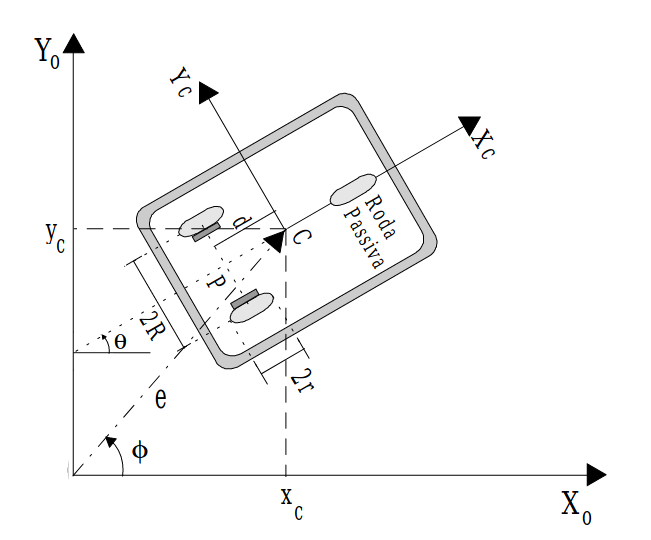
\includegraphics[width=0.8\textwidth]{capitulos/robo_dif_coordenadas.png}
    \caption{Robô diferencial em sistema de coordenadas cartesianas. \cite{sousa2003controle}}
    \label{fig:robo_coordenada_cart}
\end{figure}
\begin{figure}[ht]
    \centering
    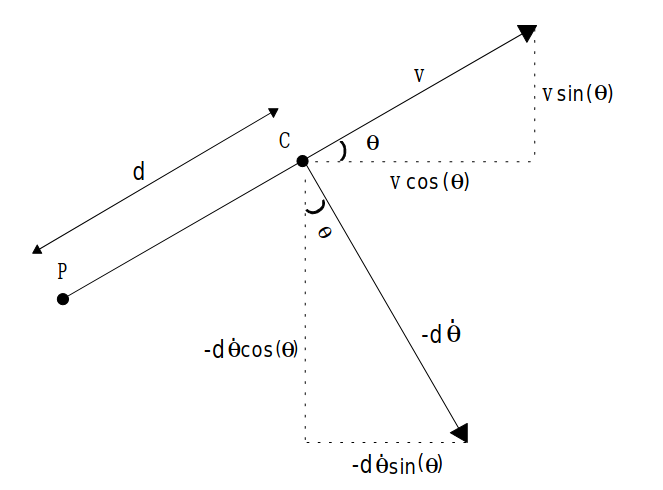
\includegraphics[width=0.8\textwidth]{capitulos/robo_dif_vetorial.png}
    \caption{Diagrama vetorial do robô diferencial, mostrando os vetores de velocidade. \cite{sousa2003controle}}
    \label{fig:robo_coordenada_vet}
\end{figure}
Ampliando a visão do modelo cinemático, pode-se visualizar a equação que rege as velocidades do robô diferencial através da Figura \ref{fig:robo_coordenada_vet}. Podemos escrever a equação através de:
\begin{equation}
  \begin{cases}
     \dot{x_{c}} = cos(\theta)v - dsin(\theta)\omega\\
     \dot{y_{c}} = sin(\theta)v + dcos(\theta)\omega\\
     \dot{\theta} = \omega
  \end{cases}
  \label{eq:1}
\end{equation},
ou, em forma matricial
\begin{equation}
    \begin{bmatrix}
       \dot{x_{c}} \\
       \dot{y_{c}} \\
       \dot{\theta}
     \end{bmatrix} = \begin{bmatrix}
       cos(\theta) & -dsin(\theta)\\
        sin(\theta) & dcos(\theta)\\
       0 & 1
     \end{bmatrix}\begin{bmatrix}
       v\\
       \omega\\
     \end{bmatrix}
     \label{eq:2}
\end{equation},
onde $v$ é a velocidade linear e $\omega$ a velocidade angular. \cite{sousa2003controle}
Com o modelo apresentado na Equação \ref{eq:2} é possível realizar o controle das variáveis de saída, $v$ e $w$, de acordo com os parâmetros de entrada que indicam a posição do robô $x, y$ e $\theta$.
\par
Outra forma de representar a cinemática direta de um robô diferencial é utilizando coordenadas polares. \cite{aicardi1995closed} Onde a representação cartesiana pode ser transformada nas variáveis $(e, \phi, \alpha)$ que podem ser descritas por:
\begin{equation}
  \begin{cases}
     e = \sqrt{x_{c}^2 + y_{c}^2}\\
     \phi = arctan2(y_{c},x_{c})\\
     \alpha = \theta - \phi
  \end{cases}
  \label{eq:3}
\end{equation}
e também, $x_{c} e y_{c}$ podem ser escritos como:
\begin{equation}
  \begin{cases}
     x_{c} = e cos(\phi)\\
     y_{c} = esin(\phi)\\
  \end{cases}
  \label{eq:4}
\end{equation}
Desta forma, é possível realizar o controle através dos parâmetros $e$, que representa o módulo da posição do robô e o parâmetro $\alpha$, que representa a orientação do robô em relação ao eixo cartesiano definido pelo sistema.
\section{Controle PID}
O algoritmo de controle PID é utilizado em larga escala para processos que necessitem de controle por realimentação, sejam eles industriais, residenciais ou afins. \cite{astrom1995}
\par
\subsection{Controle Realimentado}
O PID funciona através do principio de realimentação, que pode ser definido como: "O acréscimo da variável manipulada quando a variável de processo é menor do que o setpoint e o decréscimo da variável manipulada quando a variável de processo é maior do que o setpoint."  Utilizando este princípio, vários modelos de controladores foram criados, sendo o mais simples deles o controle on-off, que possui um sinal de controle discreto de ligado ou desligado, e o mais utilizado sendo o PID. \cite{astrom1995}

\begin{figure}[ht]
    \centering
    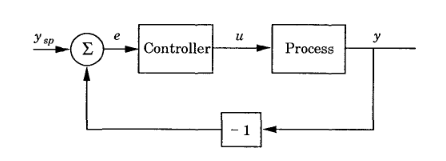
\includegraphics[width=0.8\textwidth]{capitulos/processo_feedback.png}
    \caption{Diagrama de blocos de um processo realimentado simples. \cite{astrom1995}}
    \label{fig:processo_feedback}
\end{figure}
\subsection{Elemento Proporcional, Integral e Derivativo de um PID}
Um controlador PID pode ser dividido em três partes: Proporcional, integral e derivativa. Cada uma destas partes possui uma influência em como o controlador vai alterar a resposta do sistema. \cite{ogata2011engenharia} Nesta seção cada uma delas será discutida de forma separada.
\subsubsection{Parte Proporcional}
A parte proporcional do controlador pode ser descrita pela equação: 
\begin{equation}
    u(t) = K e(t)
\end{equation}
Onde o sinal de saída $u(t)$ é proporcional ao sinal de erro $e(t)$ junto a um ganho $K$, chamado de ganho proporcional. Ou seja, o controlador proporcional apenas amplifica o sinal de controle em relação ao erro. \cite{ogata2011engenharia}

\begin{figure}[ht]
    \centering
    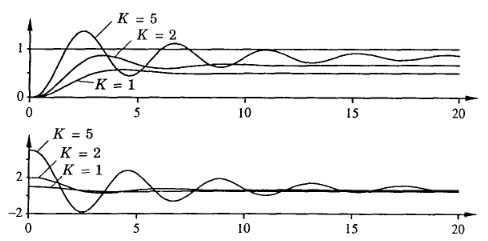
\includegraphics[width=0.8\textwidth]{capitulos/acao_controle_proporcional.png}
    \caption{Gráfico demonstrando o sinal de saída de um controlador proporcional com diferentes valores de K. \cite{astrom1995}}
    \label{fig:acao_controle_proporcional}
\end{figure}
\subsubsection{Parte Integral}
A ação integral do controlador tem a função de realizar uma somatória dos erros do sistema afim de permitir que o mesmo, em regime permanente, seja zerado.\cite{ogata2011engenharia} Sua equação é:
\begin{equation}
    u(t) = K_{i} \int_0^t e(t) dx
\end{equation}
Onde $K_{i}$ é um ganho ajustável.

\begin{figure}[ht]
    \centering
    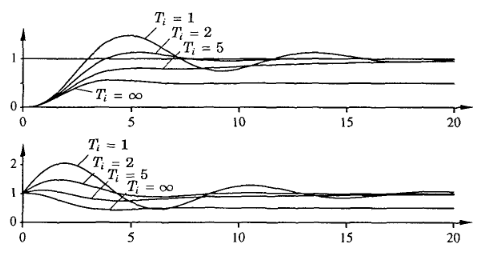
\includegraphics[width=0.8\textwidth]{capitulos/acao_controle_integral.png}
    \caption{Gráfico demonstrando o sinal de saída de um controlador integral com diferentes valores de $K_{i}$. \cite{astrom1995}}
    \label{fig:acao_controle_integral}
\end{figure}
\subsubsection{Parte Derivativa}
Já a parte derivativa possui o objetivo de realizar a previsão do erro que acontece no controlador, diminuindo o tempo que o sistema leva para se estabilizar.\cite{ogata2011engenharia} Sua componente é:
\begin{equation}
    u(t) = K_{d} \frac{de(t)}{dt}
\end{equation}

\begin{figure}[ht]
    \centering
    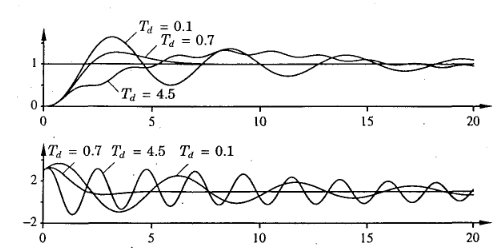
\includegraphics[width=0.8\textwidth]{capitulos/acao_controle_derivativo.png}
    \caption{Gráfico demonstrando o sinal de saída de um controlador derivativo com diferentes valores de $K_{d}$. \cite{astrom1995}}
    \label{fig:acao_controle_derivativo}
\end{figure}
\subsection{Controlador PID}
O controlador PID tradicional é a junção dos três termos citados acima, se tornando um controlador robustos para trabalhar com problemas que precisam possuir erro nulo em regime permanente e também chegar na estabilidade mais rapidamente.\cite{ogata2011engenharia} Ou seja, o PID tradicional é:
\begin{equation}
    u(t) = K_{p} e(t) + K_{i} \int_0^t e(t) dx + K_{d} \frac{de(t)}{dt}
\end{equation}
Cuja descrição em diagrama de blocos está demonstrada na Figura \ref{fig:representacao_pid}.
\begin{figure}[ht]
    \centering
    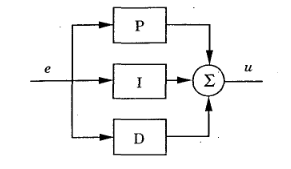
\includegraphics[width=0.5\textwidth]{capitulos/representacao_pid.png}
    \caption{Representação de diagrama de blocos de um controlador PID, separado por suas três componentes. \cite{astrom1995}}
    \label{fig:representacao_pid}
\end{figure}
\subsection{Sintonização de Controladores PID}
Para que o controlador PID consiga cumprir seu objetivo corretamente é muito importante que seus ganhos $K_{p}$, $K_{i}$ e $K_{d}$ sejam corretamente definidos. Esse projeto do controlador pode se utilizar de diversos métodos. Quando a planta é relativamente simples, sua função de transferência pode ser definida e métodos de analíticos de projetos podem ser utilizados. Entretanto, quando a planta envolve mais complexidade e não é possível separar de forma precisa a relação entre as variáveis físicas, deve-se realizar a sintonia através de regras definidas em literatura ou métodos numéricos, utilizadas inclusive em controladores PID inteligentes que conseguem realizar a sua própria sintonia fina de forma automática. \cite{ogata2011engenharia}
\par
Uma dos métodos de sintonia mais difundidas na literatura é o de  Ziegler-Nichols. O método se baseia no regime transitório da planta para encontrar o ganho proporcional $K_{p}$, o tempo integral $T_{i}$ e o tempo derivativo $T_{p}$. Esses parâmetros podem ser obtidos através da aplicação de um degrau unitário (Figura \ref{fig:resposta_degrau_unitario}  na entrada da planta e da análise na curva de resposta do sinal. Para a utilização do método, alguns critérios devem ser satisfeitos:
\begin{figure}[ht]
    \centering
    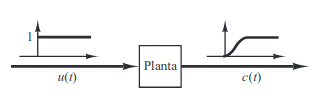
\includegraphics[width=0.5\textwidth]{capitulos/resposta_degrau_planta.png}
    \caption{Aplicação de um degrau unitário.\cite{ogata2011engenharia}}
    \label{fig:resposta_degrau_unitario}
\end{figure}
    \begin{itemize}
        \item A planta não poderá possuir integradores ou polos complexos conjugados dominantes.
        \item A resposta gráfica do sistema deverá aparentar possuir uma forma em S
    \end{itemize}
    Satisfeitos esses dois requisitos, é possível obter os valores de $L$, denominado atraso do sistema, e $T$, a constante de tempo. Essas duas constantes são obtidas através do tracejado da linha tangente à inflexão que ocorre na curva em S, vide Figura \ref{fig:curva_projeto_pid}, e identificando os pontos onde a linha cruza o eixo temporal e o eixo do ganho $K$. . 
    \begin{figure}[ht]
        \centering
        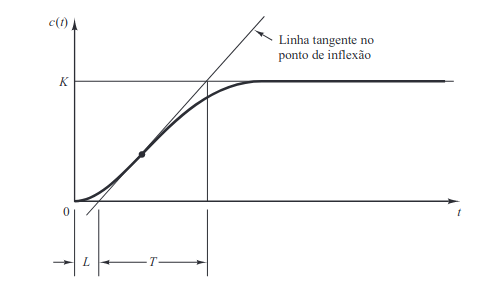
\includegraphics[width=0.5\textwidth]{capitulos/curva_projeto_pid.png}
        \caption{Análise da resposta ao degrau.\cite{ogata2011engenharia}}
        \label{fig:curva_projeto_pid}
    \end{figure}\par
    Através das duas constantes, Ziegler e Nichols propuseram a tabela \ref{tab:tabela_ziegler_nichols}, mostrada abaixo para encontrar os parâmetros $K_{p}$, $T_{i}$ e $T_{i}$.
    \begin{table}[h!]
        \centering
        \begin{tabular}{| r | c | c | c |}
        \hline
            Tipo de controlador & $K_{p}$ & $T_{i}$ & $T_{d}$ \\
            \hline
            P & $\frac{T}{L}$ & $\infty$ & $0$ \\
            \hline
            PI & $0,9\frac{T}{L}$ & $\frac{L}{0,3}$ & $0$ \\
            \hline
            PID & $1,2\frac{T}{L}$ & $2L$ & $0,5L$ \\
        \hline
        \end{tabular}
        \caption{Regra de Ziegler-Nichols}
        \label{tab:tabela_ziegler_nichols}
    \end{table}
    \par
    Desta forma, o controlador PID fica da forma
    \begin{equation}
        G_{c}(s)= K_{p} (1 + \frac{1}{T_{i}S} + T_{d}S)
    \end{equation}
\section{Visão Computacional}
\subsection{Aquisição de Imagens}
\subsection{Processamento de Imagens}
\section{Laboratórios Remotos Didáticos}
\subsection{Tipos}
\subsection{Didática}
\subsection{Estrutura e Arquitetura}
